%
% hochpass.tex -- Bild zum Thema Optische Fouriertransformation <opt>
%
% (c) 2023 Marco Niederberger, Yanick Schoch; OST Ostschweizer Fachhochschule
%

\documentclass[tikz]{standalone}
\def\skala{0.25}

\begin{document}

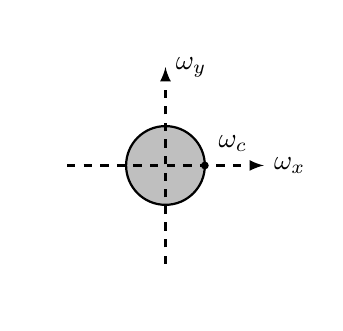
\begin{tikzpicture}[>=latex,thick,scale=\skala]
    \draw[draw=none] circle (7); %Make drawing symmetric

    \draw[draw,fill=lightgray,] circle (2);
    
    \node[label={45:{$\omega_c$}}, circle, fill, inner sep=1pt] at (2, 0) {};
    
    % x and y axis
    \draw[->, dashed] (-5,0)--(5,0) node[right]{$\omega_x$};
    \draw[->, dashed] (0,-5)--(0,5) node[right]{$\omega_y$};

\end{tikzpicture}
\end{document}
